\tab Pentru a demonostra \textbf{resetarea unui commit anterior} voi crea 2 versiuni : \textbf{FirstVersion} si \textbf{SecondVersion}. In prima voi include fisierul \textbf{newFileToRevert.txt} si voi face commit pe Git, iar intr-a doua versiune,voi sterge acel fisier si din nou commit!\\
Apoi utilizind comanda \textbf{git log} putem vedea codul,autorul si timpul fiecarui commit facut. Vom copia primele 7 cifre ale codului pe care le vom introduce in urmatoarea comanda \textbf{git reset --hard ******* }\\
Ulterior vom observa un mesaj care ne informeaza ca acum suntem la FirstVersion cu codul indicat anterior.\\
PEntru verificare vom introduce comanda \textbf{ls} pentru a ne afisa lista de fisiere. Astfel vom vedea ca fisierul care a fost sters in versiunea a doua va aparea din nou,ceea ce demonstreaza ca am revenit la prima versiune cu siguranta!\\

\begin{figure}[h]
\centering
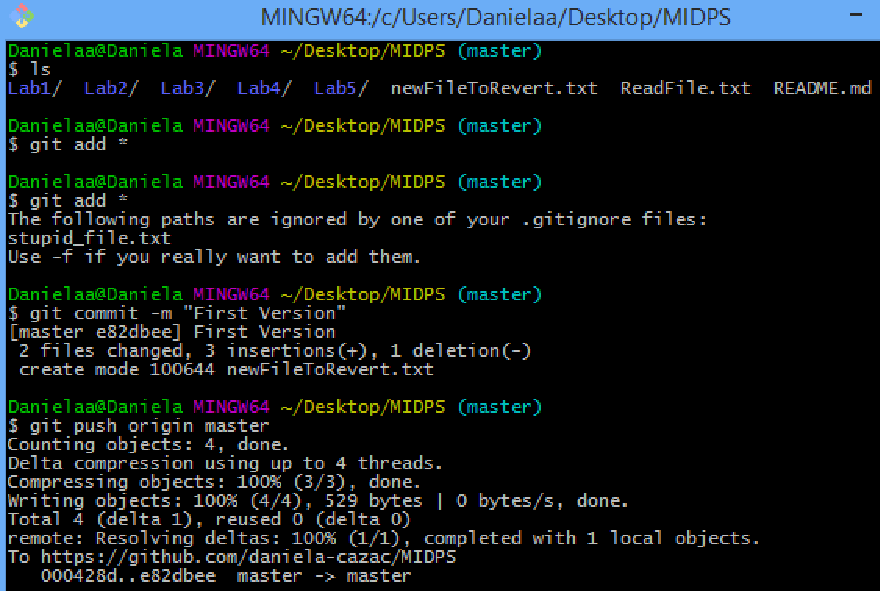
\includegraphics[scale=1]{FirstVersion}
\end{figure}
\clearpage

\begin{figure}[h]
\centering
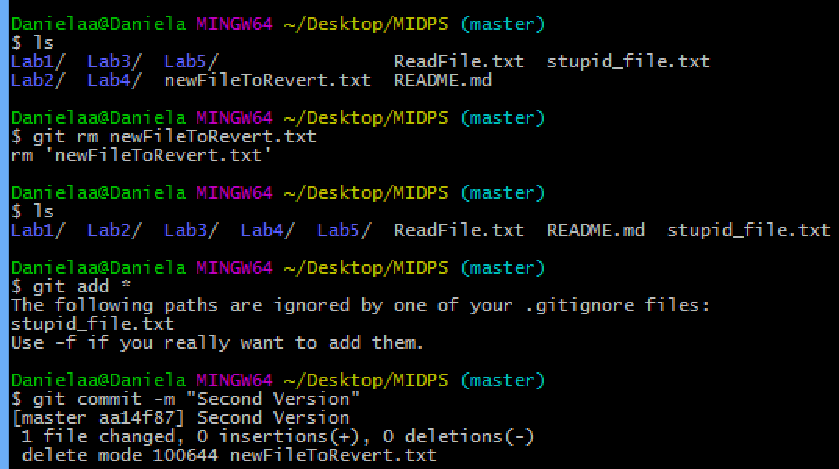
\includegraphics[scale=1]{SecondVersion}
\end{figure}
\begin{figure}[h]
\centering
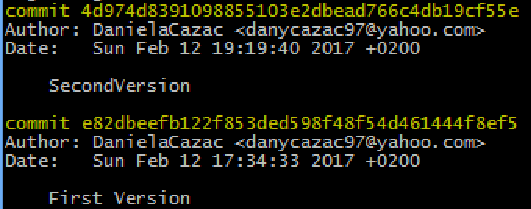
\includegraphics[scale=1]{gitLog}
\end{figure}
\begin{figure}[h]
\centering
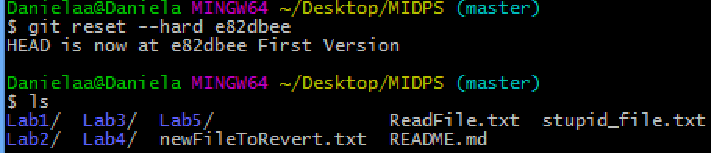
\includegraphics[scale=1]{reset}
\end{figure}

\clearpage
\clearpage